\documentclass[12pt]{article}
\usepackage[margin=1in]{geometry} 
\usepackage{amsmath,amsthm,amssymb,amsfonts}
\usepackage[colorlinks=true]{hyperref} 
\usepackage{graphicx}
\graphicspath{ {images/} }
 
\newcommand\tab[1][1cm]{\hspace*{#1}}
\newcommand{\N}{\mathbb{N}}
\newcommand{\Z}{\mathbb{Z}}
 
\newenvironment{problem}[2][Problem]{\begin{trivlist}
\item[\hskip \labelsep {\bfseries #1}\hskip \labelsep {\bfseries #2.}]}{\end{trivlist}}
%If you want to title your bold things something different just make another thing exactly like this but replace "problem" with the name of the thing you want, like theorem or lemma or whatever

\begin{document}
 
%\renewcommand{\qedsymbol}{\filledbox}
%Good resources for looking up how to do stuff:
%Binary operators: http://www.access2science.com/latex/Binary.html
%General help: http://en.wikibooks.org/wiki/LaTeX/Mathematics
%Or just google stuff
 
\title{ASTR 512 Extragalactic \\ Problem Set \# 1 Solutions}
\author{N. Nicole Sanchez}
\maketitle
 
\begin{problem}{1} 
I would like to select ``Cold gas in galaxies''\tabularnewline as my specialization topic. \\

I've selected the following top 5 papers: \\
\tab \href{http://adsabs.harvard.edu/abs/2006MNRAS.365...11C}{Croton et. al. 2006} \\
\tab \href{http://adsabs.harvard.edu/abs/2005MNRAS.363....2K}{Kere\^s et. al. 2005} \\
\tab \href{http://adsabs.harvard.edu/abs/2004ApJ...613..898T}{Tremonti et. al. 2004} \\ 
\tab \href{http://adsabs.harvard.edu/abs/1997ApJ...490..493N}{Navarro et. al. 1997} \\
\tab \href{https://arxiv.org/pdf/0808.0553.pdf}{Dekel et. al. 2009} \\

I am currently reading Kere\^s et. al. 2005 and \href{https://arxiv.org/pdf/1510.05650.pdf}{Hayward et. al. 2017} (for Journal Club).
\end{problem}
 
\begin{problem}{2}
I'm very glad the NED Database search came before the Classifying Galaxies. It was a far more efficient way of finding the real T-Types of the galaxies I was classifying.
\end{problem}

\pagebreak

\begin{problem}{3}
\end{problem}

\begin{figure}[ht!]
\vspace{-3 mm}
\centerline{\resizebox{0.85\hsize}{!}{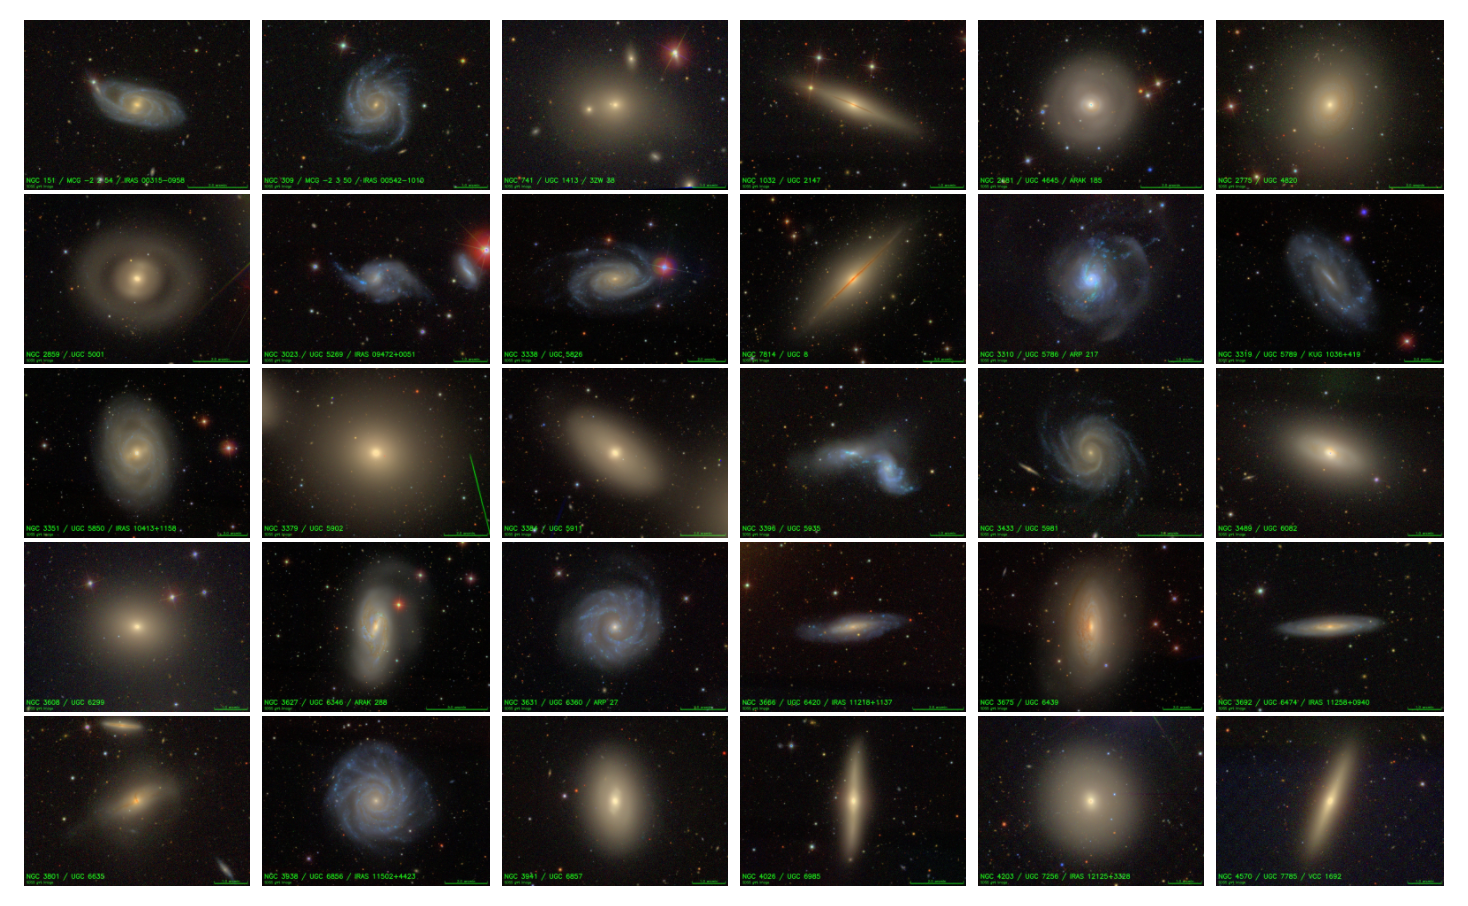
\includegraphics[angle=0]{classifiedgalaxies.png}}}
\caption[]{The 30 galaxies classified in Figure \ref{galplots}.}
\label{galclass}
\end{figure}

\begin{figure}[ht!]
\centerline{\resizebox{1.1\hsize}{!}{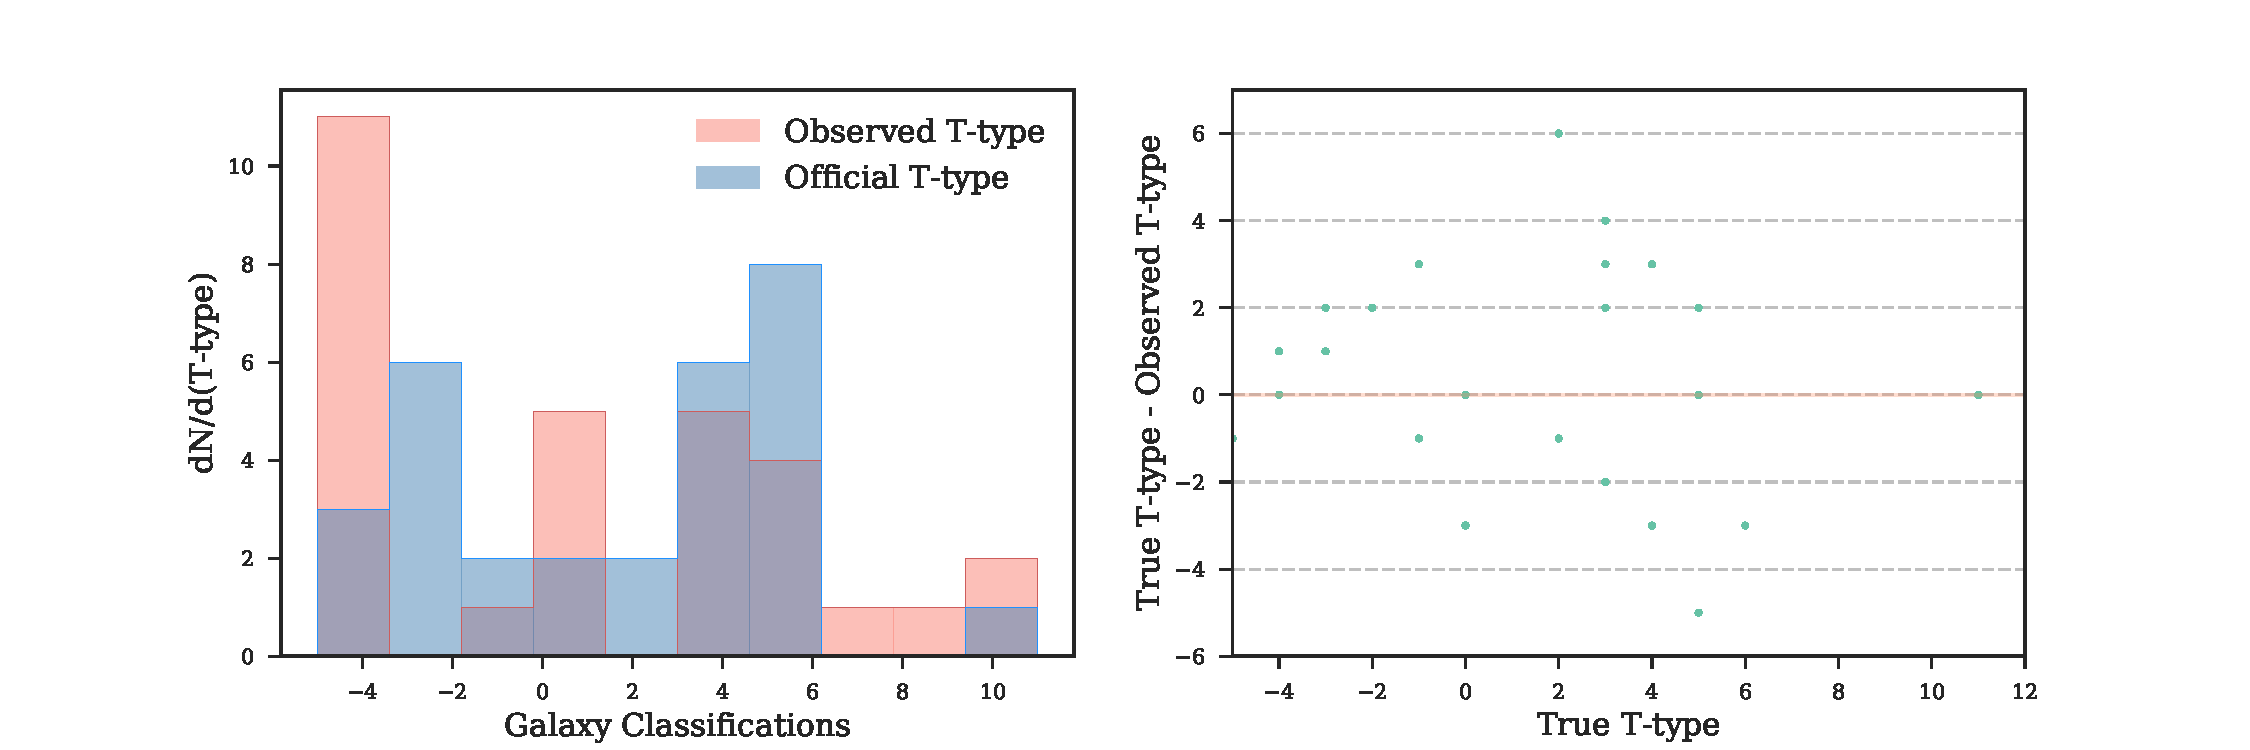
\includegraphics[angle=0]{gxy_class_hist.pdf}}}
\caption[]{$Left:$ Histogram of my observed galaxy classification (and corresponding T-Types) and the true T-Types for the 30 galaxies in Figure \ref{galclass}. $Right:$ The difference between True and Observerd galaxy T-Types as a function of their True T-Types.}
\label{galplots}
\end{figure}

\textbf{Biases:} My classifications tended to trend as Elliptical galaxies. When the official classification was often closer to an S0/a or S0 +/−+/− , I would be more likely to classify it as an Elliptical galaxy. I also classified my spiral galaxies more broadly, more often classifying them as c/d than the official classifications.

 \pagebreak
\begin{problem}{4}
\end{problem}

\begin{figure}[ht!]
\centerline{\resizebox{1.2\hsize}{!}{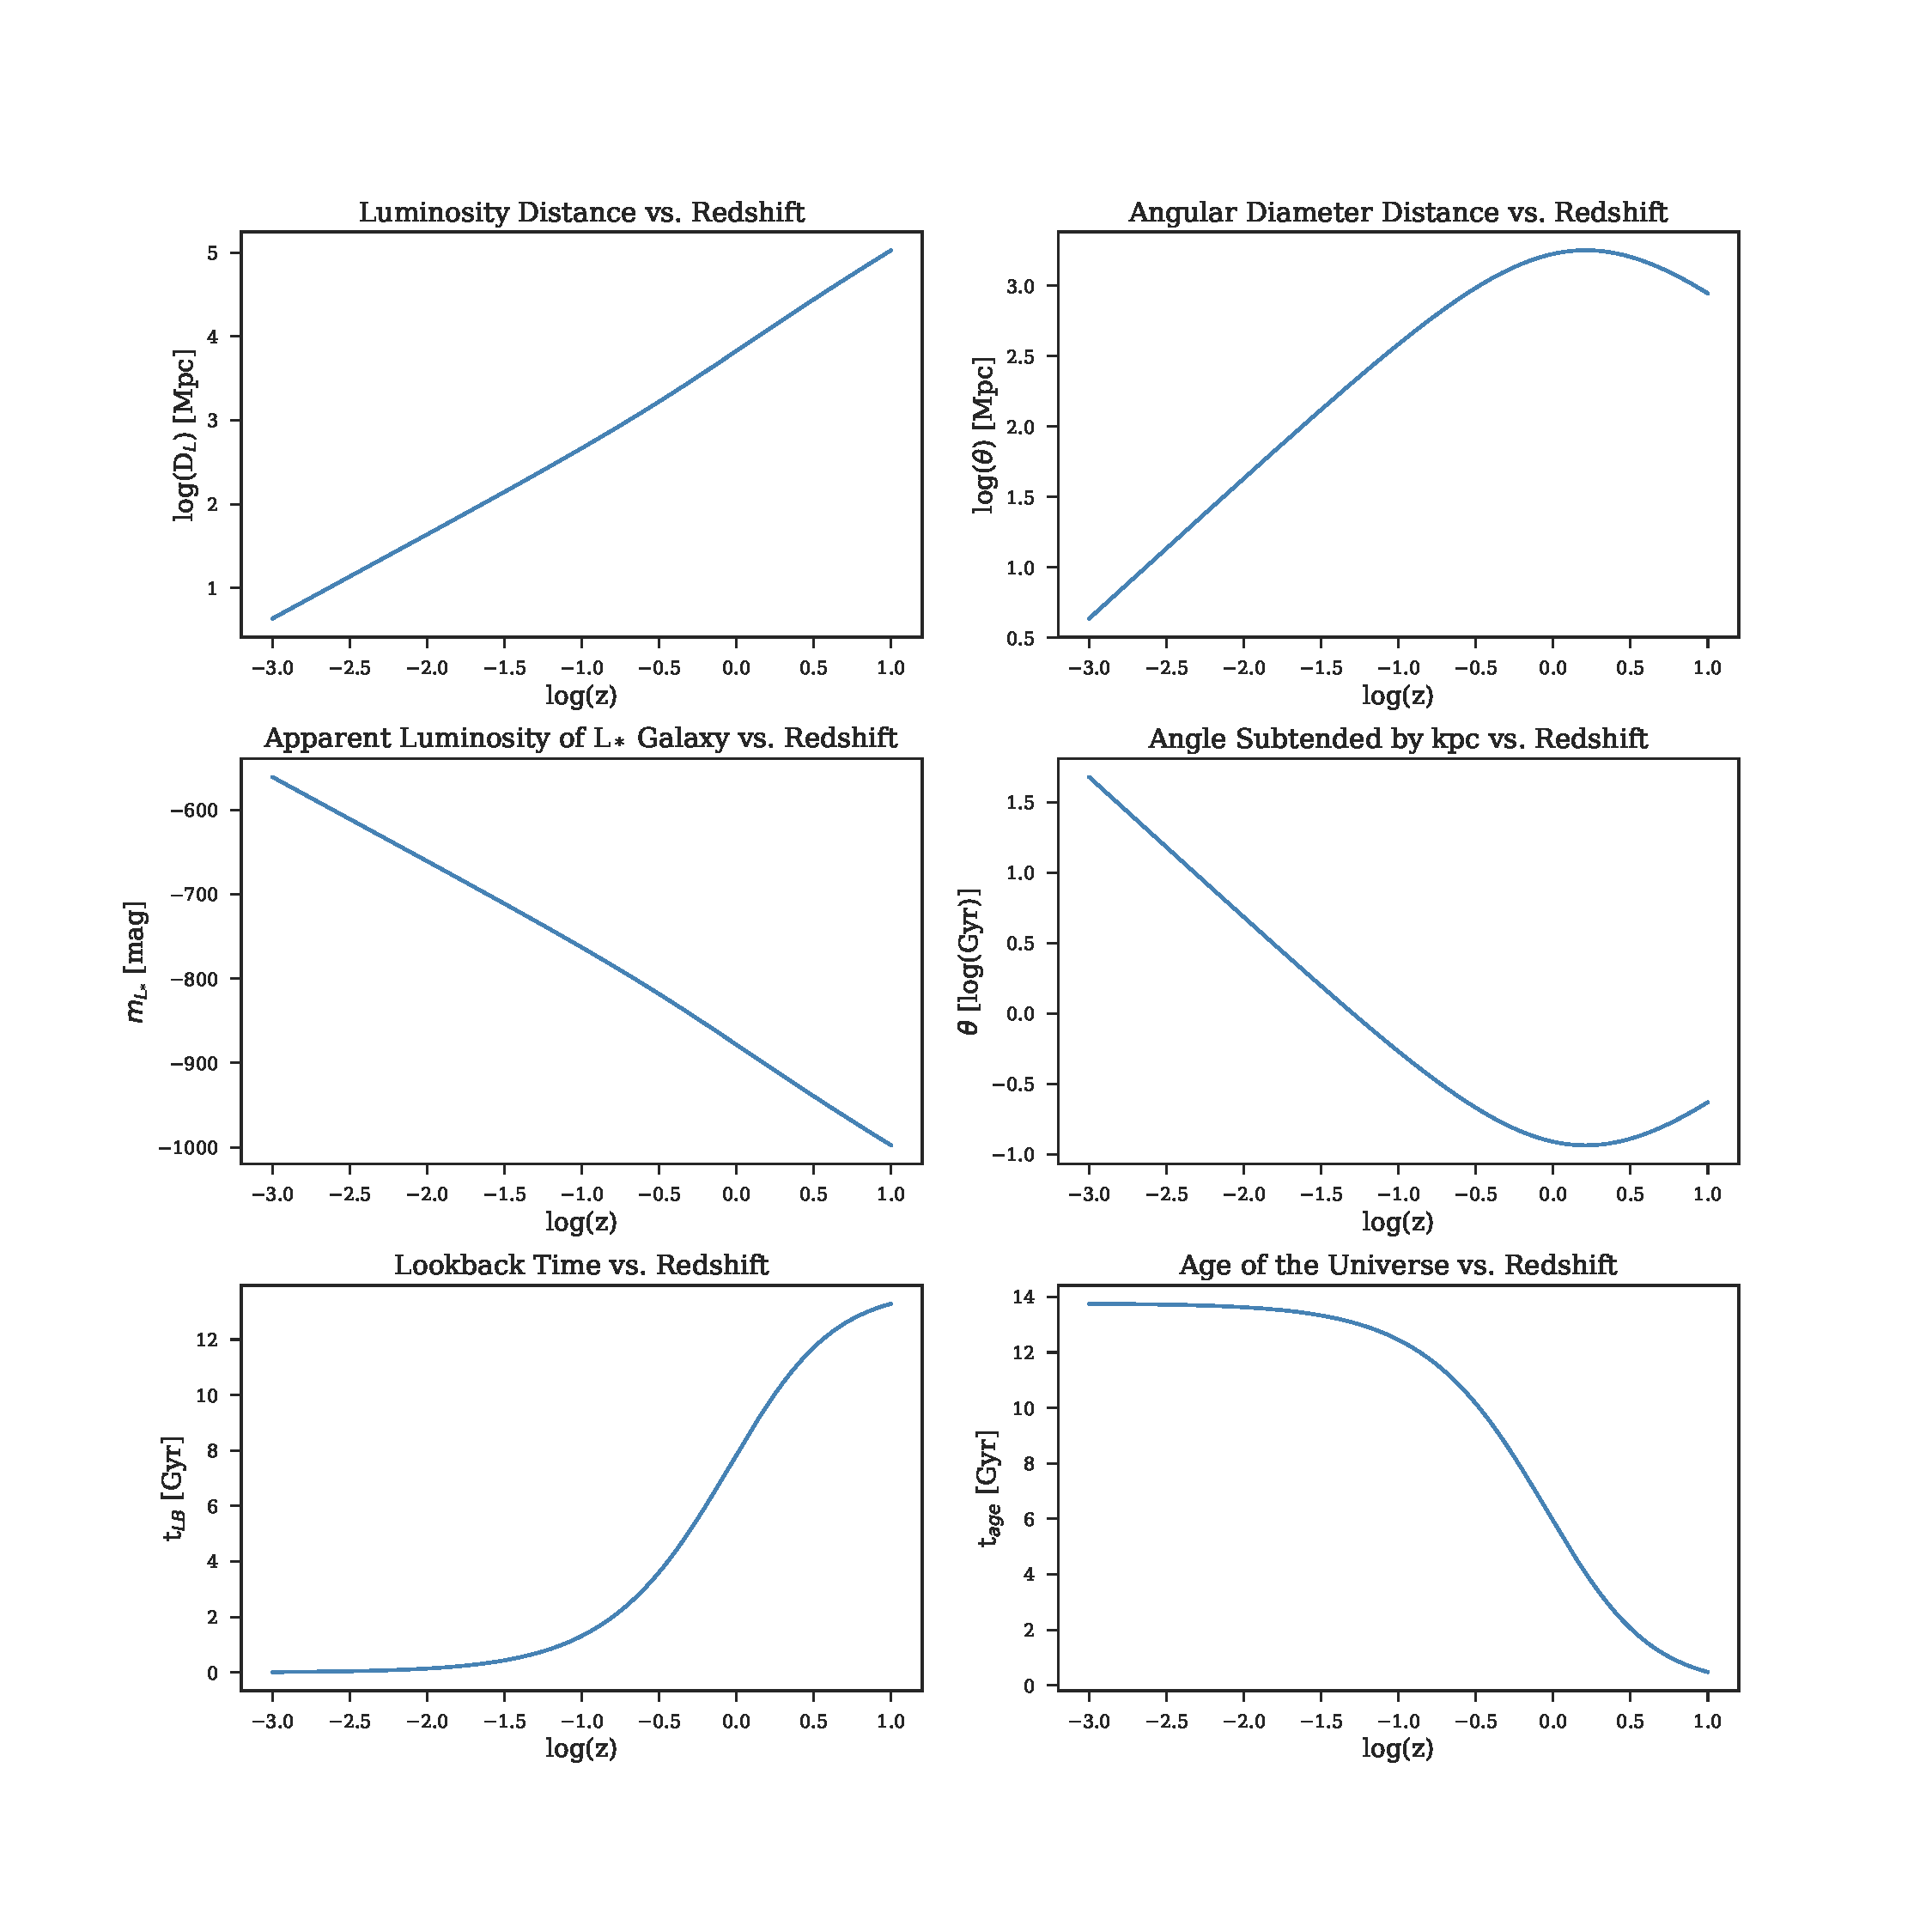
\includegraphics[angle=0]{xtrgxy_scales.pdf}}}
\caption[]{Plots of extragalactic scales as a function of redshift.}
\label{xscale}
\end{figure}

\begin{figure}[ht!]
\tab \centerline{\resizebox{1.\hsize}{!}{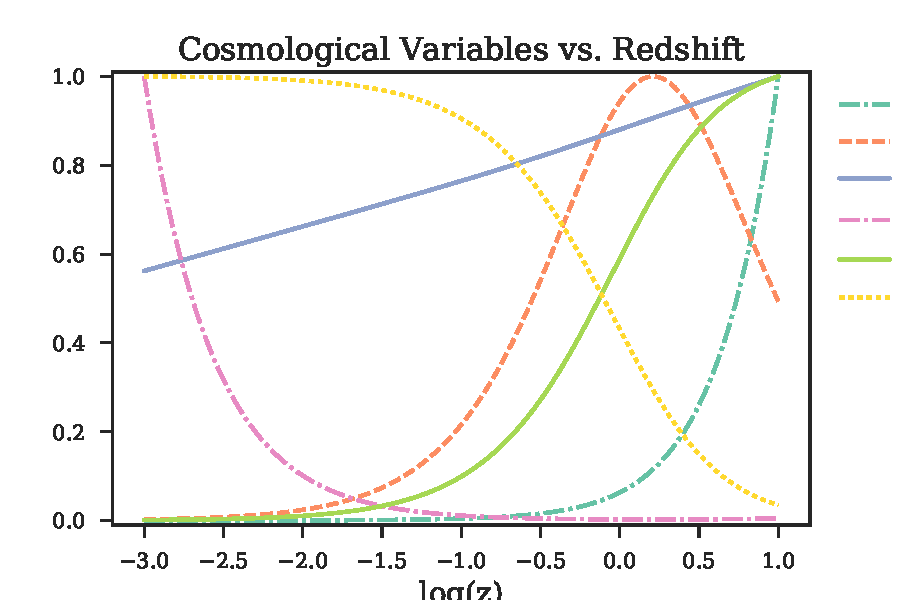
\includegraphics[angle=0]{xtrgxy_scales2.pdf}}}
\caption[]{All extragalactic scales normalized to one and plotted against redshift.}
\label{xscale2}
\end{figure}

\end{document}